\chapter{Metodologia}

Este capítulo define, de forma preliminar, a metodologia que será seguida durante o desenvolvimento do trabalho e está sujeita a mudanças conforme coleta e análise dos documentos acadêmicos.

\section{Visão Geral da Metodologia}

A metodologia proposta tem como base uma abordagem de aprendizado não-supervisionado e detecção de anomalias através da análise e extração multimodal. Busca-se rotular documentos com base em um nível de probabilidade de fraudulência, para isso, utilizam-se extrações de características visuais (como textura, fonte, espaçamento, selos e assinaturas), textuais (como padrões linguísticos, formatação de números e distribuição de termos) e estruturais (como posição de campos, margens e tabelas), que serão refinadas conforme realização do TCC. Combinando essas \textit{features} multidimensionais, é possível realizar o agrupamento dos documentos em \textit{clusters} que representam padrões dominantes normais. Em sequência, modelos de detecção de anomalias são utilizados para a criação de detectores de referência a partir dos \textit{clusters}, possibilitando a classificação de um novo documento submetido, em tempo real, através da avaliação do grau de desvio em relação aos padrões aprendidos — quanto maior o desvio e escore de anomalia, maior a probabilidade de que o documento seja falsificado. Finalmente, essa pontuação é mapeada para categorias discretas de suspeita, fornecendo um nível de probabilidade de fraude para cada inserção. O processo completo consiste em duas etapas: treinamento dos modelos de referência e classificação de novos documentos.

A escolha dessa abordagem tem por base a premissa de que documentos falsificados apresentam inconsistências sutis, tornando-os atípicos em relação aos padrões estabelecidos por documentos legítimos, sendo detectáveis através da análise multimodal das características extraídas de diversos contextos.

\subsection{Treinamento dos Modelos de Referência}

Representada na Figura \ref{fig:fluxotreino}, a fase de treinamento inicia com a coleta de certificações acadêmicas diversas, seguida do pré-processamento através de técnicas de normalização de imagens e aplicação de OCR. Com o \textit{dataset} formado, é realizada a extração e processamento multimodal de características visuais, textuais e estruturais dos documentos. Em sequência, com base nos dados obtidos na etapa anterior, é realizada a identificação de padrões utilizando algoritmos de \textit{clustering} para identificar grupos de documentos com comportamentos similares, estabelecendo padrões dominantes de normalidade. Por fim, detectores de anomalias são treinados para cada padrão descoberto, gerando modelos de referência normais.

\begin{figure}[H]
	\caption{\label{fig:fluxotreino}Representação do Fluxo de Treino}
    \begin{center}
    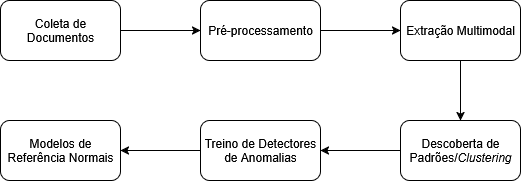
\includegraphics[width=.9\linewidth]{images/FluxoTreino.png}
	\end{center}
	\fonte{o autor}
\end{figure}

\subsection{Classificação de Novo Documento}

Representada na Figura \ref{fig:fluxoanalise}, o processo de classificação de novo documento utiliza os modelos de referência estabelecidos na fase de treinamento para determinar a probabilidade de falsificação.

\begin{figure}[H]
	\caption{\label{fig:fluxoanalise}Representação do Fluxo de Análise de Novo Documento}
    \begin{center}
    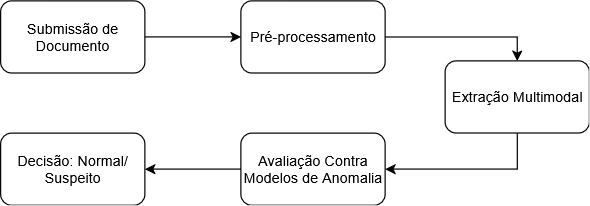
\includegraphics[width=.9\linewidth]{images/FluxoAnalise.png}
	\end{center}
	\fonte{o autor}
\end{figure}

O processo inicia com a submissão de um novo certificado e, para garantir consistência na representação das características, passa pelo mesmo \textit{pipeline} de pré-processamento e extração multimodal utilizado na fase de treinamento. Em seguida, os dados de representação do documento, obtidos na etapa anterior, são comparados contra todos os modelos de referência normal. Cada modelo calcula um escore de anomalia baseado na distância, ou similaridade, em relação ao padrão estabelecido pelo modelo. Essas pontuações representam, por fim, a probabilidade de falsificação do registro. Finalmente, utilizam-se métricas de consenso para categorizar o arquivo, isto é, classificá-lo como normal ou suspeito a partir de determinado limiar de pontos.

\subsection{Extração Multimodal de Características}

O módulo de extração multimodal, utilizado tanto no fluxo de treino quanto no fluxo de classificação de uma submissão, é responsável por capturar diferentes aspectos dos documentos. Essa abordagem permite aproveitar o mesmo \textit{pipeline} de processamento combinando características independentes e, no contexto deste trabalho, complementares. Busca-se poder detectar tanto falsificações grosseiras quanto sofisticadas, uma vez que mesmo contrafações bem-feitas tendem a apresentar inconsistências sutis.

\begin{figure}[H]
	\caption{\label{fig:fluxomultimodal}Representação do Fluxo de Extração Multimodal de Características}
    \begin{center}
    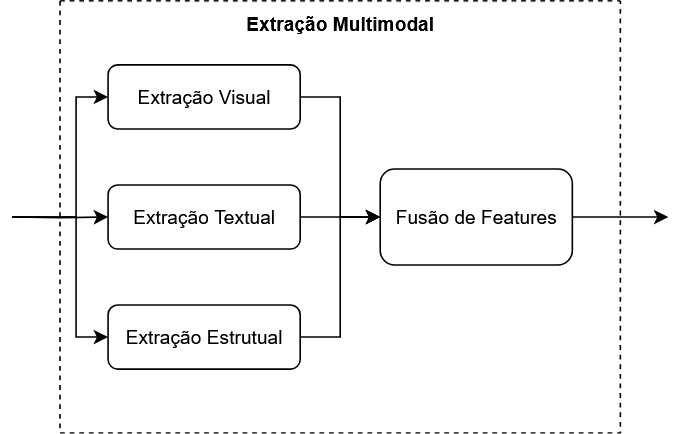
\includegraphics[width=1\linewidth]{images/FluxoExtracao.png}
	\end{center}
	\fonte{o autor}
\end{figure}

Ao invés de focar em características de domínios específicos, como nos trabalhos correlatos, essa abordagem combina três diferentes subprocessos de extração de \textit{features} em paralelo, como representado na Figura \ref{fig:fluxomultimodal}:

\begin{itemize}
    \item Extração visual: extrai características ligadas ao layout, qualidade e consistência visual dos documentos. Inclui análise de textura, propriedades de fonte (espessura, tamanho, espaçamento), qualidade de assinaturas e selos, resolução de imagem, e padrões de cores e contrastes;
    \item Extração textual: utiliza modelos de processamento de linguagem natural para extrair características linguísticas e de formatação. Analisa padrões textuais, distribuição de termos, consistência na formatação de números, datas e códigos, além de verificar a coerência semântica do conteúdo;
    \item Extração estrutural: extrai características ligadas à organização espacial e estrutural dos documentos. Examina posicionamento de campos, formatação de tabelas, alinhamentos, margens, espaçamentos e a disposição geral dos elementos no documento.
\end{itemize}

Por fim, é realizada a fusão das características extraídas em todos os subprocessos. Para isso, os dados são normalizados e são aplicadas técnicas de redução dimensional, evitando a \textit{maldição da dimensionalidade}, o que resulta em uma representação completa, unificada e compacta de cada documento.